\chapter{Примеры вычисления работы силы. Работа силы тяжести, линейной силы
упругости и силы тяготения.}

\section{Работа силы тяжести}
Пусть точка \( M \), на котороую действует сила тяжести \( \vec{P} \), 
перемещается из положения \( M_0(x_0, y_0, z_0) \) в положение 
\( M_1(x_1, y_1, z_1) \). Выберем координатные оси так, чтобы ось \( Oz \) 
была направлена вертикально вверх (рис. \ref{pic52_01}). Тогда 
\( P_x = 0, P_y = 0, P_z = -P \). Подставляя эти значения в формулу:
\[ 
    A_{(M_0 M_1)} = \int_{(M_0)}^{(M_1)} 
    \left( F_x dx + F_y dy + F_z dz \right) \quad (52.1)
\]
получим, учитывая, что переменным интегрирования является \( z \):
\[ 
    A_{(M_0 M_1)} = - \int_{z_0}^{z_1} Pdz = 
    P\left(z_0 - z_1 \right) 
\]

\begin{figure}[h!]
    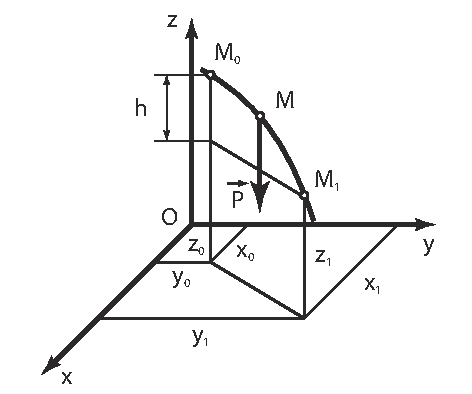
\includegraphics[width=.47\textwidth]{52_01}\hfill
    \parbox{.47\textwidth}{\caption{} \label{pic52_01}}
\end{figure}

Если точка \( M_0 \) выше \( M_1 \), то \( z_0 - z_1 = h \), где 
\( h \) -- вертикальное перемещение точки; если же точка \( M_0 \) ниже 
точки \( M_1 \), то \( z_0 - z_1 = -\left(z_1 - z_0\right) = -h \).

Окончательно получаем \( A_{(M_0 M_1)} = \pm Ph \).

Из полученного результата следует, что работа силы тяжести не зависит от 
вида той траектории, по которой перемещается точка её приложения.

\section{Работа линейной силы упругости}
Рассмотрим груз \( M \), лежащий на горизонтальной плоскости и 
прикрепленный к свободному концу некоторой прижины (рис. \ref{pic52_02}). На 
плоскости отметим точку \( O \) положение, занимаемое концом пружины, 
когда она не напряжена (\( AO = l_0 \) -- длина ненапряженной пружины), и 
примем эту точку за начало координат. Если теперь оттянуть груз от 
равновесного положения \( O \), растянув пружину до величины \( l \), то
пружина получит удлинение \( k = l - l_0 \) и на груз будет действовать 
силу упругости \( \vec{F} \), направленная к точке \( O \). Так как в 
нашем случае \( k = x \), то по формуле \( F = ck \) 
(\( k \) -- удлинение (или сжатие) пружиныж; \( с \) -- коэффициент 
жёсткости пружины):
\[ F = ck = c|x| \text{ и } F_x = -cx \]
Последнее равенство справедливо и при \( x < 0 \) 
(груз левее точки \( O \); тогда сила \( \vec{F} \) направлена вправо и 
получится, как и должно быть, \( F_X > 0 \).

\begin{figure}[h!]
    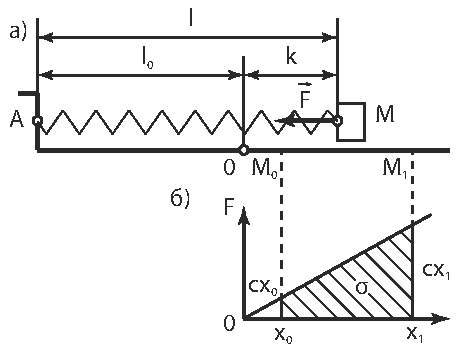
\includegraphics[width=.47\textwidth]{52_02}\hfill
    \parbox{.47\textwidth}{\caption{} \label{pic52_02}}
\end{figure}

Найдём работу, совершаемую силой упругости при перемещении груза из 
положения \( M_0(x_0) \) в положение \( M_1(x_1) \). Так как в данном 
случае \( F_x = -cx, F_y = F_z = 0 \), то, подставляя эти значения в 
формулу (52.1), найдём
\[ 
    A_{(M_0 M_1)} = - \int_{x_0}^{x_1} cxdx = 
    \frac{c}{2} \left( x^{2}_0 - x^{2}_1 \right) 
\]

\emph{Этот же результат можно получить по графику зависимости 
\( F \) от \( x \) (рис \ref{pic52_02}), вычисляя площадь \( \sigma \) 
заштрихованной на чертеже трапеции и учитывая знак работы.}

В полученной формуле \( x_0 \) представляет собой начальное удлинение 
пружины \( k_0 \), а \( x_1 \) -- конечное удлинение пружины \( k_1 \). 
Следовательно, 
\[ A_{(M_0 M_1)} = \frac{c}{2} \left( k^{2}_0 - k^{2}_1 \right) \]
то есть \emph{работа силы упругости равна половине произведения 
коэффициента жёсткости на разность квадратов начального и конечного 
удлинения (или сжатий) пружины.}

\section{Работа силы тяготения}
Если Землю (планету) рассматривать как однородный шар (или шар, 
состоящий из однородных концентрических слоёв), то на точку \( M \) с 
массой \( m \), находящуюся вне шара на расстоянии \( r \) от его 
центра \( O \) (или находящуюся на поверхности шара), будет действовать 
сила тяготения \( \vec{F} \), направленная к центру \( O \) (рис. \ref{pic52_03}), 
значение которой определяется формулой \( F = fm_1 m_2 / r^2 \) 
( \( f \) -- гравитационная постоянная \). Представим эту формулу в виде: 
\[ F = \frac{km}{r^2} \]
и определим коэффициент \( k \) из того условия, что, когда точка 
находится на поверхности земли ( \( r = R \), где \( R \) -- радиус Земли), 
сила притяжения равна \( mg \), где \( g \) -- ускорение силы тяжести 
(точнее силы тяготения) на земной поверхности. Тогда должно быть
\[ mg = \frac{km}{R^2} \text{ и } k = gR^2 \]

\begin{figure}[h!]
    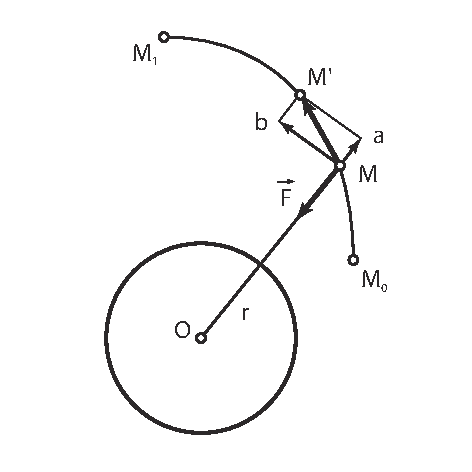
\includegraphics[width=.47\textwidth]{52_03}\hfill
    \parbox{.47\textwidth}{\caption{} \label{pic52_03}}
\end{figure}

Подсчитаем сначала элементарную работу силы \( \vec{F} \). Как видно из 
рисунка, элементарное перемещение \( \vec{MM'} \) точки \( M \) можно 
разложить на перемещение \( \vec{Ma} \), численно равное приращению 
\( dr \) расстояния \( OM = r \) и направленное вдоль \( OM \), и на 
перемещение \( \vec{Mb} \), перпендикулярное \( OM \), а следовательно, и 
силе \( \vec{F} \). Поскольку на втором перемещении работа силы 
\( \vec{F} \) равна нулю, а перемещение \( \vec{Ma} \) направлено 
противоположно силе, то 
\[ dA = -Fdr = -km\frac{dr}{r^2} = -mgR^2 \frac{dr}{r^2} \]

Допустим теперь, что точка перемещается из положения \( M_0 \), где 
\( r = r_0 \), в положение \( M_1 \), где \( r = r_1 \). Тогда 
\[ 
    A_{(M_0 M_1)} = \int_{(M_0)}^{(M_1)} dA = 
    -mgR^2 \int_{r_0}^{r_1} \frac{dr}{r^2} =
    mgR^2 \int_{r_0}^{r_1} d\left( \frac{1}{r} \right)
\]
или окончательно
\[ A_{(M_0 M_1)} = mgR^2 \left( \frac{1}{r_1} - \frac{1}{r_0} \right) \]

\newpage
